% !TEX program = xelatex
\documentclass[12pt]{ctexart}
% ------------------------
% 页面
% ------------------------
\usepackage{geometry}
\geometry{margin=2.5cm}

% ------------------------
% 字体
% ------------------------
\usepackage{fontspec}
\setmainfont{Segoe UI}
\setmonofont{Consolas}

% ------------------------
% 基础包
% ------------------------
\usepackage{multirow}
\usepackage{soul}
\usepackage[normalem]{ulem}
\usepackage{lastpage}
\usepackage{xcolor}
\usepackage{hyperref}
\usepackage{graphicx}
\usepackage{booktabs}
\usepackage{enumitem}
\usepackage{caption}
\usepackage{titlesec}
\usepackage{fancyhdr}
% ------------------------
% GitHub 颜色
% ------------------------
\definecolor{gh-bg}{HTML}{FFFFFF}
\definecolor{gh-border}{HTML}{D0D7DE}
\definecolor{gh-codebg}{HTML}{F6F8FA}
\definecolor{gh-link}{HTML}{0969DA}
\definecolor{gh-line}{HTML}{8B949E}

\definecolor{gh-note}{HTML}{0969DA}
\definecolor{gh-warning}{HTML}{9A6700}
\definecolor{gh-tip}{HTML}{1A7F37}

% ------------------------
% 设置页眉与页尾
% ------------------------
\geometry{left=2cm,right=2cm,top=2cm,bottom=2.5cm}
\fancyhf{}
\fancyhead[C]{}
\fancyhead[L]{中国科学院大学·2026年春}
\fancyhead[R]{网络空间安全导论}
\fancyfoot[C]{第 \thepage 页，共 \pageref{LastPage} 页}
\renewcommand{\footrulewidth}{0.4pt}
\renewcommand{\baselinestretch}{1.2}
\pagestyle{fancy}
% ------------------------
% 超链接
% ------------------------
\hypersetup{
	colorlinks=true,
	linkcolor=gh-link,
	urlcolor=gh-link
}

% ------------------------
% 列表间距
% ------------------------
\setlist{
	itemsep=4pt,
	topsep=6pt
}

% ------------------------
% tcolorbox
% ------------------------
\usepackage{tcolorbox}
\tcbuselibrary{minted,skins,breakable}

% ------------------------
% GitHub 引用块
% ------------------------
\newtcolorbox{ghquote}{
	enhanced,
	colback=white,
	colframe=gh-border,
	borderline west={3pt}{0pt}{gh-border},
	arc=2pt,
	left=10pt,
	right=10pt,
	top=6pt,
	bottom=6pt
}

% ------------------------
% GitHub 提示框
% ------------------------
\newtcolorbox{note}{
	enhanced,
	colback=white,
	colframe=gh-note,
	borderline west={4pt}{0pt}{gh-note},
	title=Note
}

\newtcolorbox{warning}{
	enhanced,
	colback=white,
	colframe=gh-warning,
	borderline west={4pt}{0pt}{gh-warning},
	title=Warning
}

\newtcolorbox{tip}{
	enhanced,
	colback=white,
	colframe=gh-tip,
	borderline west={4pt}{0pt}{gh-tip},
	title=Tip
}

% ------------------------
% 代码块
% ------------------------
\usepackage{minted}

\newtcblisting{codeblock}[2][]{
	listing engine=minted,
	minted language=#2,
	minted options={
		linenos,
		breaklines,
		fontsize=\small,
		numbersep=10pt,
		xleftmargin=15pt
	},
	colback=gh-codebg,
	colframe=gh-border,
	arc=6pt,
	boxrule=0.5pt,
	left=6pt,
	right=6pt,
	top=6pt,
	bottom=6pt,
	listing only,
	breakable,
	#1
}

% ------------------------
% 行内代码
% ------------------------
\newtcbox{\inlinecode}{
	on line,
	boxrule=0pt,
	colback=gh-codebg,
	arc=4pt,
	left=3pt,
	right=3pt,
	top=2pt,
	bottom=2pt
}

% ------------------------
% 标题样式
% ------------------------
\titleformat{\section}
{\Large\bfseries}
{\thesection}{0.5em}{}

\titleformat{\subsection}
{\large\bfseries}
{\thesubsection}{0.5em}{}


\renewcommand{\theFancyVerbLine}{\color{gh-line}\small\arabic{FancyVerbLine}}

\newtheorem{application}{应用}
\newtheorem{problem}{问题}
\newtheorem{analogy}{分析}
\newtheorem{experiment}{实验}

% ------------------------
% 修改表头信息
% ------------------------
%改这里可以修改实验报告表头的信息
\newcommand{\name}{陈曦}
\newcommand{\studentNum}{2025K8009970002}
\newcommand{\boxNum}{}
\newcommand{\expNum}{ICS-exp02-00}
\newcommand{\expName}{密码学(可选)}
\newcommand{\finishdate}{2026年3月25日}

% ------------------------
% 文档开始
% ------------------------
\setlength{\headheight}{14.49998pt}
\begin{document}
	
	\begin{center}
		\LARGE 中国科学院大学·网络空间安全导论实验报告 
	\end{center}
	
	\begin{center}
		\emph{箱子号} \underline{\makebox[4em][c]{\boxNum}}
		\emph{实验序号} \underline{\makebox[8em][c]{\expNum}}
		\emph{实验专题} \underline{\makebox[16em][c]{\expName}}\\
		\emph{小组成员} \underline{\makebox[36em][c]{\name}}\\
		\emph{对应学号} \underline{\makebox[36em][c]{\studentNum}}\\
		\emph{最后修改日期} \underline{\makebox[34em][c]{\finishdate}}
		{\noindent}
		\rule[8pt]{17cm}{0.2em}
	\end{center}
	\begin{abstract}
		本实验围绕密码学的核心概念展开，首先系统梳理了密码学的发展历程，从古典密码到现代公钥密码体系，阐述了其在信息安全领域的基础性地位。在此基础上，重点分析了哈希算法与加密算法在设计目标、可逆性、输出特性及应用场景等方面的本质区别，并结合实际案例（如操作系统镜像校验、区块链工作量证明、HTTPS 协议）进行了对比说明。进一步地，本文通过 OpenSSL 与 Nginx 完成了自签名证书 HTTPS 服务器的搭建实践，验证了数字证书在传输层安全协议中的作用及其在浏览器中的呈现效果。实验结果表明，哈希算法适用于完整性校验与身份验证场景，而加密算法则侧重于数据保密与安全通信，二者在现代密码体系中各司其职、互为补充。本次实验深化了对密码学基本原理的理解，也为后续网络空间安全相关技术的学习奠定了基础。同时最后也实现了用GnuPG生成专属于自己的公钥与私钥，并将此份实验报告通过加密发送给学长
	\end{abstract}
		
	\section{背景简介}
		本次实验是密码学的第一次实验，也是第一次不需要强制要求写实验报告的一次实验。但是笔者对密码学有着充分的兴趣，我与密码学的渊源可以追溯到初中的时候，也就是差不多新冠疫情的时期。当时恰逢新冠疫情宅家学习，(PS:说是学习，其实我大部分时间都在网上漫游。)所以当时的我有了充分的时间接触互联网，也就是在那个时候，我第一次通过一个叫做回形针\footnote{[注：回形针这个UP主因为各种各样的政治站位问题目前在国内已经被ban了，因此本文仅对视频学术内容用作引用以考证笔者对密码学的兴趣来源，不对政治立场做出过多评价。\hyperlink{https://www.youtube.com/watch?v=TVlo66aOZE0}{网页连接(需要梯子)}]}的B站UP主对硬科普这个概念感兴趣。(PS:虽然后面发现也没有那么硬说是)我记得当时的时候加密货币的概念是炒的最火的时候，什么比特币，以太坊(ETH)都是资本市场上炙手可热的香饽饽。在当时，我记得回形针做了一期视频专门讲解了区块链技术背后的那个技术——哈希加密(Hash)，非对称加密，去中心化网络。因此在我看来，密码学的本质是一门强数学，同时又具有很强实用价值的学科。出于兴趣，笔者独立完成了以下关于密码学的本次可选实验。
	\section{密码学综述}
		密码学是密码的科学。从过程来看，密码学可以分成对加密与解密过程的研究；从实现来看，密码学可以分成对于密钥，算法，分发过程的研究；从历史维度来看，密码学可以分成古典密码学,近代密码学与现代密码学。
		
		古典密码学的起源很早，研究也很丰富。古希腊时期人们就使用Scytale圆木棍实现换位法加密（斯巴达棒）。随着时间推演，古典密码又催生出了替代式密码这一大流派，代表作有凯撒密码与维吉尼亚密码。查询相关资料得知\cite{gudianmima}：我国古代的密码学研究也十分丰富。古代中国在军队保密通信中发展出阴符、阴书、符契、信牌、字验等方法，其中《六韬》记载阴符八种符号对应战事信息，阴书需拆分三部分合读。从现代的眼光来看，已经出现了一定的分组密码与数字签名的思想。
		
		进入20世纪以来，随着真空电子管技术与硅基半导体技术的蓬勃发展，电子计算机技术有了很大提升，人类的算力有了很大飞跃，这为密码学技术的进一步演进提供了坚实的物质基础。1949年，C.E.香农基于其在第二次世界大战期间从事密码破译的工作实践，在1949年发表了论文《保密系统的通信理论》。该论文奠定了现代密码学的理论基础。香农首次将密码学的研究置于严格的信息论框架之下，提出了混淆与扩散两大设计原则，并明确了密码体制的完美安全性概念。这一时期的密码学开始从一门基于直觉与经验的技艺，逐步转变为一门有坚实理论支撑的系统科学。自此，密码学的\textbf{机密性，完整性，可用性}等设计理念开始萌芽。
		
		进入20世纪70年代，密码学迎来了又一次革命性的飞跃。美国国家标准局于1977年正式颁布了数据加密标准（DES），标志着密码算法开始走向标准化与商业化。更为关键的是，1976年，W. Diffie与M. Hellman发表了论文《密码学的新方向》，首次提出了公钥密码的思想，打破了长期以来对称密码体制的局限。这一思想随后于1978年由R. Rivest、A. Shamir与L. Adleman通过RSA算法的提出而得以具体实现，使得数字签名与密钥安全分发成为可能，开启了现代密码学的新纪元。
		
		自20世纪90年代至今，密码学的研究范畴进一步扩展与深化。随着互联网的普及与信息技术的飞速发展，密码学不再局限于传统的保密通信，而是广泛融入到网络安全、电子商务、区块链、云计算等新兴领域。分组密码与公钥密码体系不断演进，高级加密标准（AES）作为新一代对称密码标准被广泛采用。同时，哈希函数、消息认证码\cite{krawczyk1997hmac}、零知识证明\cite{goldwasser1989knowledge}、同态加密\cite{gentry2009fully}、后量子密码\cite{zong2025mathematical}等前沿方向的研究蓬勃发展，不断拓展着密码学的理论边界与应用空间。
		
		纵观密码学的发展历程，从古典密码中的简单替换与换位，到近代密码学的机械与电子化实现，再到现代密码学中基于数学难题与信息论构建的复杂体系，这一演进不仅反映了人类对信息安全需求的持续提升，也深刻体现了密码学与数学、计算机科学、物理学等多学科交叉融合的内在特征。在信息技术高度发达的今天，密码学已成为保障数字社会安全运行的基石性学科。
	\section{实验 Methods}
		\begin{problem}
			哈希 (Hashing) 与加密 (Encryption) 的本质区别是什么？请阐述两者在设计目标、核心特性（如可逆性）和典型应用场景上的根本不同。试分别举出至少两个你日常生活中会接触到的、分别应用了哈希和加密技术的例子，并说明为什么在该场景下选择的是其中一种而非另一种技术。
		\end{problem}
		\begin{analogy}
			根据相关公开资料\cite{hashwechat}，我们不难知道，对于哈希函数这种杂凑函数，其核心是一种\textbf{完全不可逆的单向门}，而这种功能与加密(一种单向陷门)而言最大的本质区别在于不可逆性。同时，Hash算法是一种摘要算法，输出的字段是定长的，这与一般的加密算法有很大区别。摘要算法的设计目标是为每一个目标生成一个独特的电子“指纹”，不同于加密算法旨在实现信息的保密性，确保只有持有正确密钥的接收方才能解读。同时从数学上也不难发现，哈希算法的密文空间的维数比明文空间的维数低，所以哈希函数本身还是具有一定的理论上的碰撞性(这也是类似哈希这样的摘要算法的共性，其中MD5摘要算法已经在王小云院士团队下发现可容易复现的碰撞性\cite{wang2005break})。而一般的加密算法要求具有完全可逆的解密算法，这种数学上的双射特征要求明文空间与密文空间线性同构，且明文与密文一一对应。综上所述的特征也导致了哈希算法的主要应用场景与加密算法不同。
			
			\begin{center}
				\textbf{表1：}Hash算法(摘要算法)与加密算法在应用场景上的区别\\
				\hspace*{2em} \\
				\begin{tabular}{ll}
					\toprule
					算法类型 & 主要应用场景\\
					\midrule
					\multirow{2}{*}{摘要算法} & 数据完整性校验、身份验证、数字指纹\\
						& 消息认证码、数据结构与快速查找等\\
					\midrule
					加密算法 & 数据保密、网络握手、密钥分发与管理、数字签名等\\
					\bottomrule
				\end{tabular}
			\end{center}
			\hspace*{2em} \\
			{\large \textbf{ 哈希算法的应用例子}}\\
			\hspace*{2em}干网安的对于Kali Linux一定不会陌生，下载系统镜像这活一定也都干过。作为一个非常注重安全的操作系统品牌，Kali Linux的官网对于下载这种与操作系统相关的“大文件”的时候是提供了SHA-256值进行校验的\\
			\hspace*{2em} \\
			\begin{minipage}{\columnwidth}
				\begin{center}
					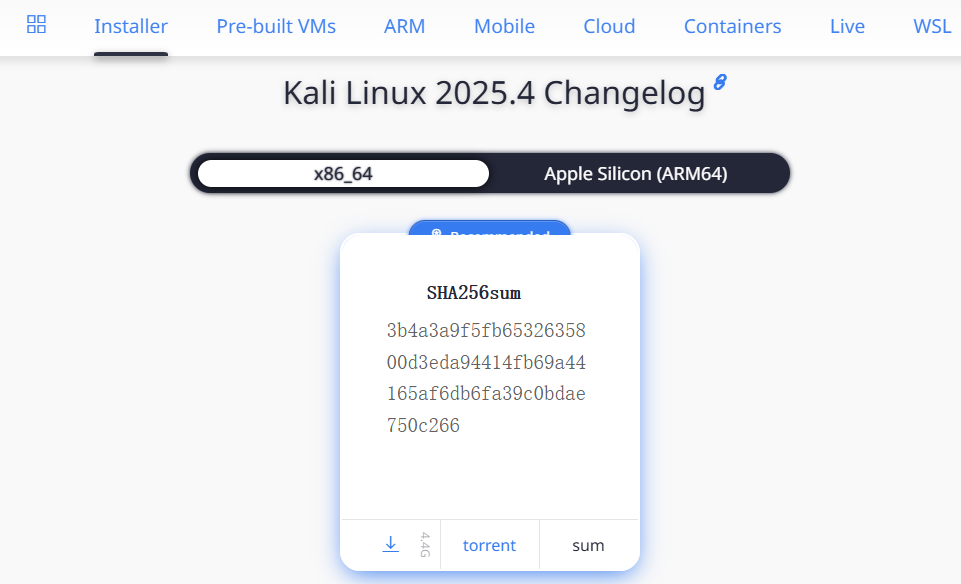
\includegraphics[width=0.5\columnwidth]{pngs/kali-hash.png}\\
					\textbf{图1：}下载镜像文件的时候提供Hash值进行校验
				\end{center}
			\end{minipage}
			\hspace*{2em}\\
			毕竟，假如往操作系统中藏毒的话，这种危害就不小了。
			
			另外一个例子就是像比特币这样的加密货币，他基于区块链的技术，采用一种叫做工作量证明(Proof of Work)的模式，本质上就是让一群人一起暴力破解计算一个哈希值，看谁算的快，算的快的就可以把算出来的区块连接到公链上，最终完成交易链条。比如下面这个交易网站展示了一个刚刚挖出来的区块\href{https://www.blockchain.com/explorer}{https://www.blockchain.com/explorer}\\
			\begin{minipage}{\columnwidth}
				\begin{center}
					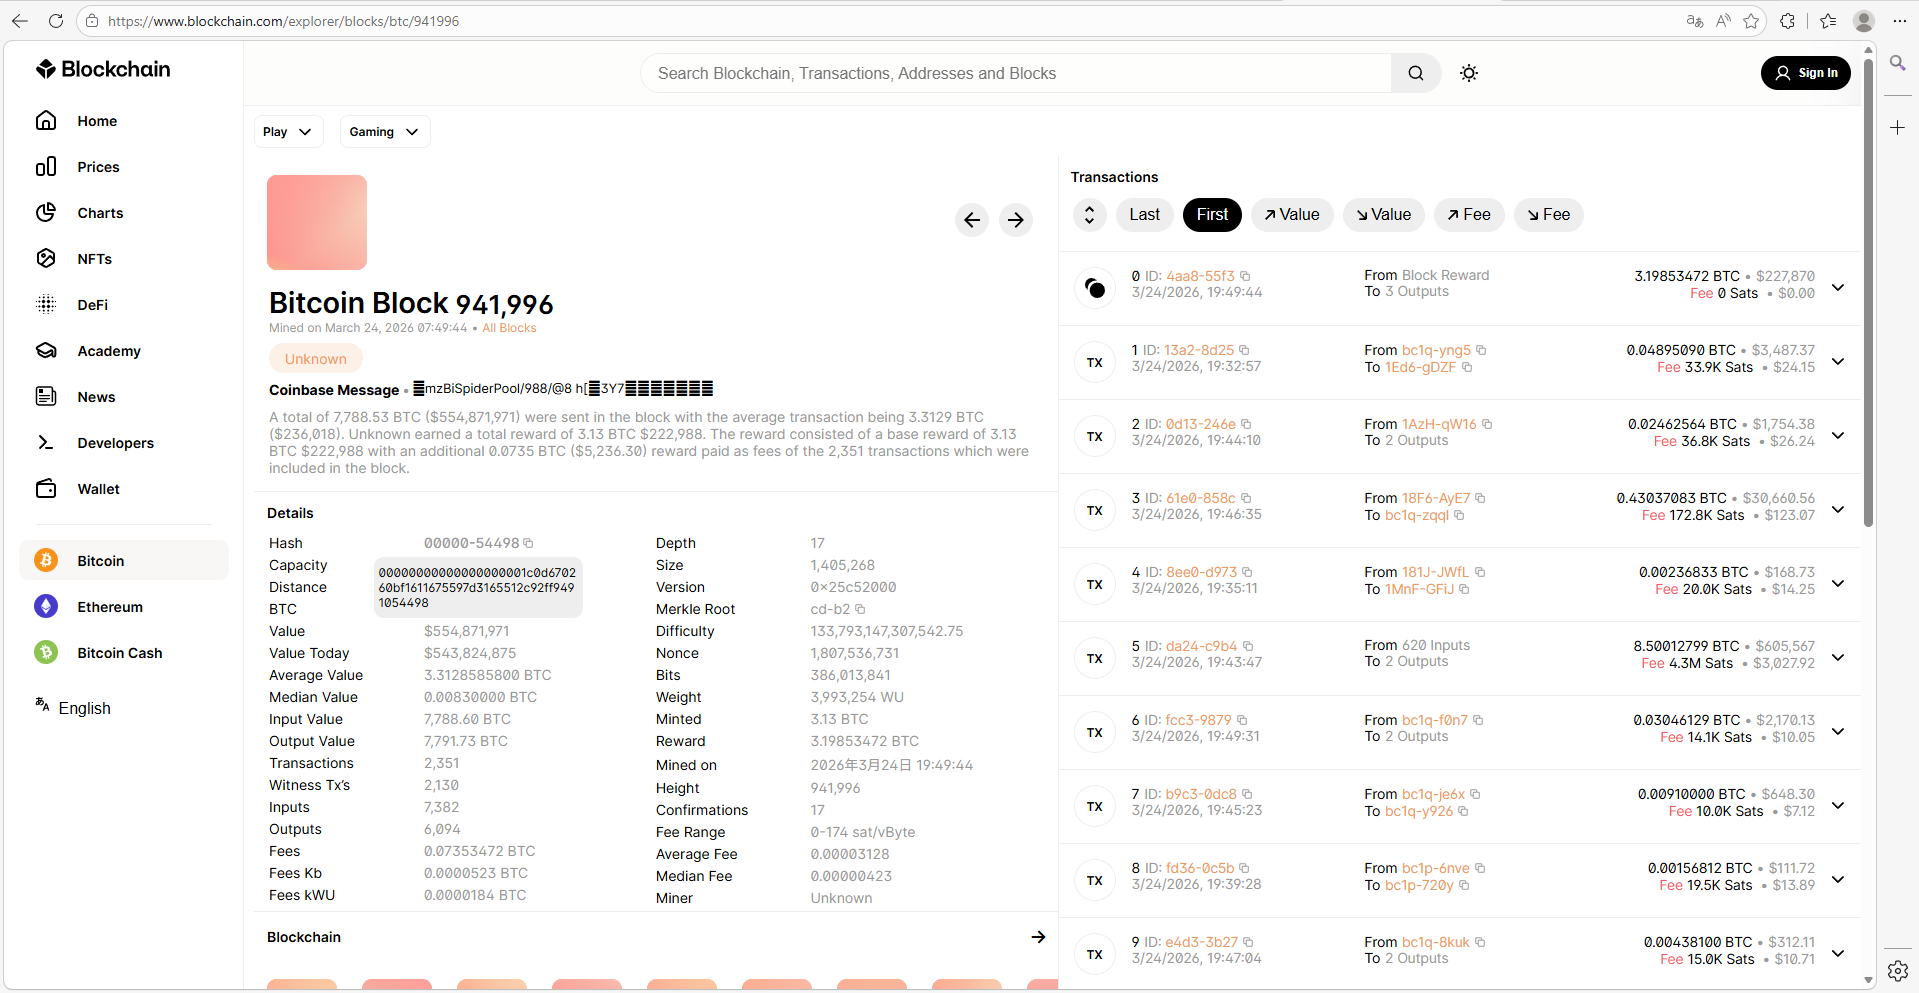
\includegraphics[width=0.8\linewidth]{pngs/full-hash.png}\\
					\textbf{图2：}一个在2026年3月24日晚上23：06上刚刚挖出来的哈希值\\
				\end{center}
			\end{minipage}
			{\large \textbf{加密算法的例子}}\\
			\hspace*{2em}比如说我后面用nginx搭建的简单版本的网页浏览器，使用wireshark捕获分析，分别使用HTTP头与HTTPS头访问网站的抓包效果是不一样的\\
			\begin{minipage}{\columnwidth}
				\begin{center}
					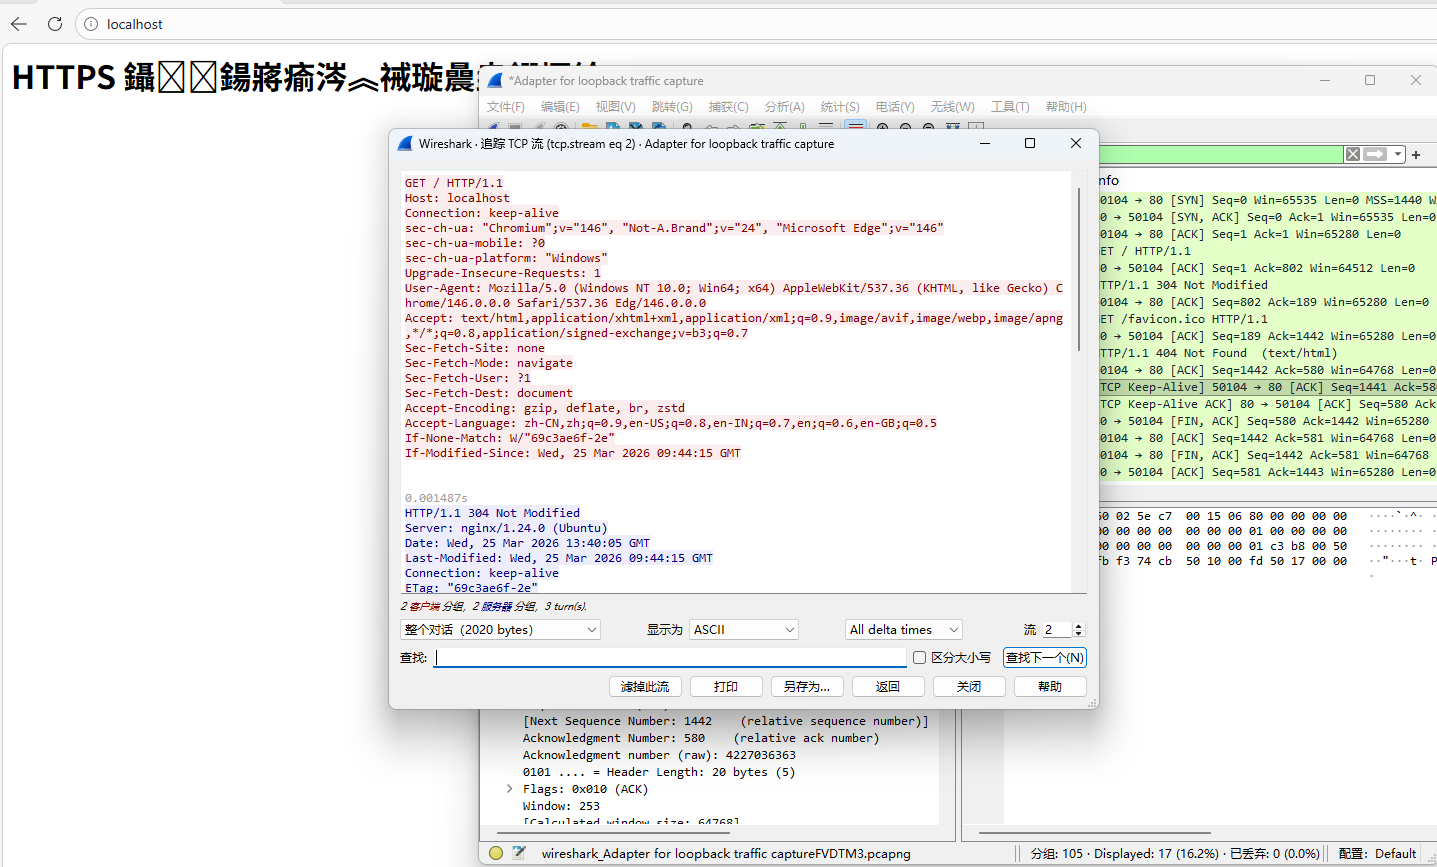
\includegraphics[width=0.4\linewidth]{pngs/http.png}\\
					\textbf{图3：}使用HTTP协议访问
				\end{center}
			\end{minipage}
			\hspace*{2em}使用HTTP协议访问是不会使用加密措施的，所以使用wireshark可以很清晰地捕获到请求头等相关信息，但是换用HTTPS协议之后，数据流就变成了下面这个鬼样子\\
			\begin{minipage}{\columnwidth}
				\begin{center}
					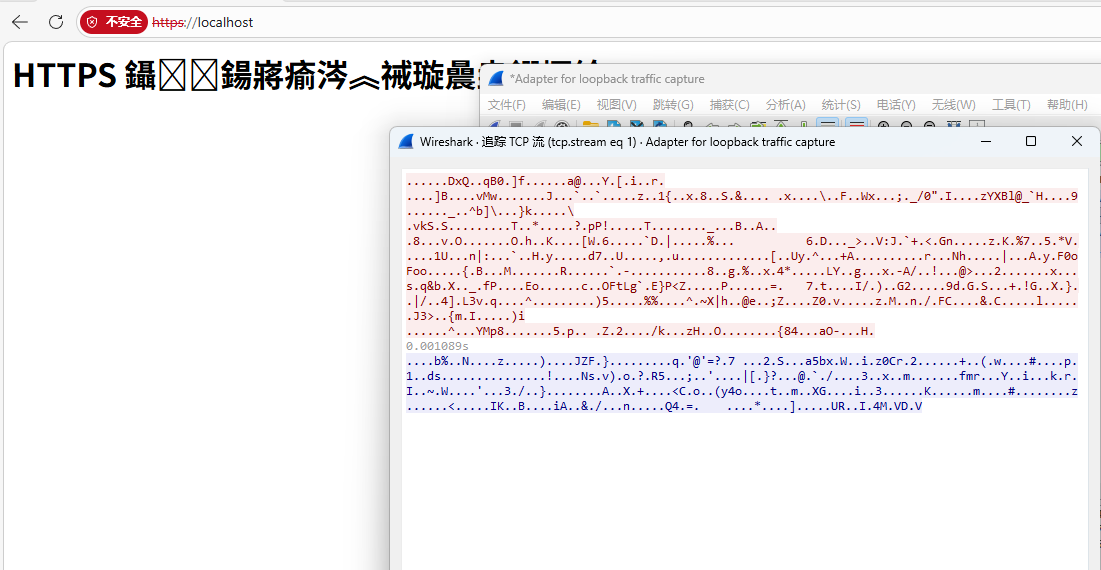
\includegraphics[width=0.4\linewidth]{pngs/https.png}\\
					\textbf{图4：}使用HTTPS协议访问
				\end{center}
			\end{minipage}
			\hspace*{2em}
		\end{analogy}
		\begin{problem}
			进阶探究：配置自签名证书HTTPS服务器
		\end{problem}
		\begin{analogy}
			OpenSSL是一个强大的加密库，广泛应用于互联网的各个角落，用于保护数据传输的安全。它实现了SSL和TLS协议，这些协议是现代网络安全的基石。而这种基础的握手协议，是当今以用户/服务器为核心架构的互联网时代的压舱石。通过配合使用OpenSSL工具与nginx、apache 或 caddy 等 HTTP 服务中间件，配置其支持HTTPS，我们可以搭建一个最小版本的服务器
			
			通过查询相关资料得知\cite{openssl}，首先创建自签名证书
			\begin{codeblock}{bash}
# 在当前文件夹(/mnt/c/users/CX\_incommand/)下创建一个存放密钥的文件夹
mkdir web
cd web

# 然后生成私钥与自签名证书
openssl req -x509 -newkey rsa:2048 -keyout server.key -out server.crt -days 365 -nodes
			\end{codeblock}
			\begin{center}
				\textbf{表2：}参数说明\\
				\hspace*{2em}\\
				\begin{tabular}{ll}
					\toprule
					参数 & 说明\\
					\midrule
					\inlinecode{req} & 证书请求及生成工具\\
					\inlinecode{-x509} & 输出自签名证书（不生成请求，直接输出证书）\\
					\inlinecode{-newkey rsa:2048} & 生成一个新的 2048 位 RSA 私钥\\
					\inlinecode{-keyout server.key} & 私钥保存文件名\\
					\inlinecode{-out server.crt} & 证书保存文件名\\
					\inlinecode{-days 365} & 证书有效期为365天\\
					\inlinecode{-nodes} & 不对私钥进行加密\\
					\bottomrule
				\end{tabular}
			\end{center}
			执行命令后，会提示输入证书信息（国家、省份、城市、组织、通用名称等）。通用名称（Common Name）必须填写服务器的域名或 IP，由于是本地测试，可以填写 \inlinecode{localhost} 或 \inlinecode{127.0.0.1}
			\begin{minipage}{\columnwidth}
				\begin{center}
					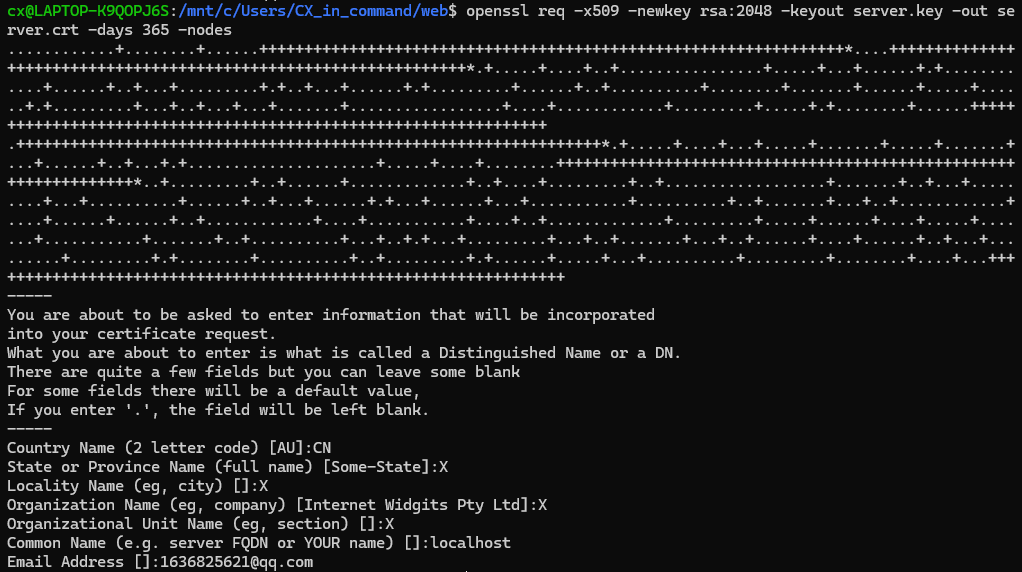
\includegraphics[width=0.7\linewidth]{pngs/crt.png}\\
					\textbf{图5：}openssl控制台输出
				\end{center}
			\end{minipage}
			接下来使用 Nginx进行配置，首先安装
			\begin{codeblock}{bash}
sudo apt update
sudo apt install nginx
			\end{codeblock}
			然后在\inlinecode{/etc/nginx/sites-available/}下创建一个配置文件\inlinecode{http\_test}
			\begin{codeblock}{bash}
sudo nano /etc/nginx/sites-available/https_test
			\end{codeblock}
			内容如下
			\begin{codeblock}{nginx}
server{
    listen 443 ssl;
    server_name localhost;

    ssl_certificate /mnt/c/Users/CX_in_command/web/server.crt;
    ssl_certificate_key /mnt/c/Users/CX_in_command/web/server.key;

    root /var/www/html;
    index index.html index.htm;

    location / {
        try_files $uri $uri/ =404;
    }
}
			\end{codeblock}
			启用站点
			\begin{codeblock}{bash}
sudo ln -s /etc/nginx/sites-available/https_test /etc/nginx/sites-enabled/
			\end{codeblock}
			然后测试配置并重启 Nginx
			\begin{codeblock}{bash}
sudo nginx -t                 # 测试配置文件语法
sudo systemctl reload nginx   # 重载配置
			\end{codeblock}
			在默认根目录 /var/www/html/ 下创建一个简单的测试页面 index.html：
			\begin{codeblock}{bash}
echo "<h1>HTTPS 自签名证书测试成功！</h1>" | sudo tee /var/www/html/index.html
			\end{codeblock}
			打开浏览器，访问 https://localhost。
			
			由于使用的是自签名证书，浏览器会显示安全警告（如“您的连接不是私密连接”）。这是正常的，因为证书未经 CA 机构签名。\\
			\begin{minipage}{\columnwidth}
				\begin{center}
					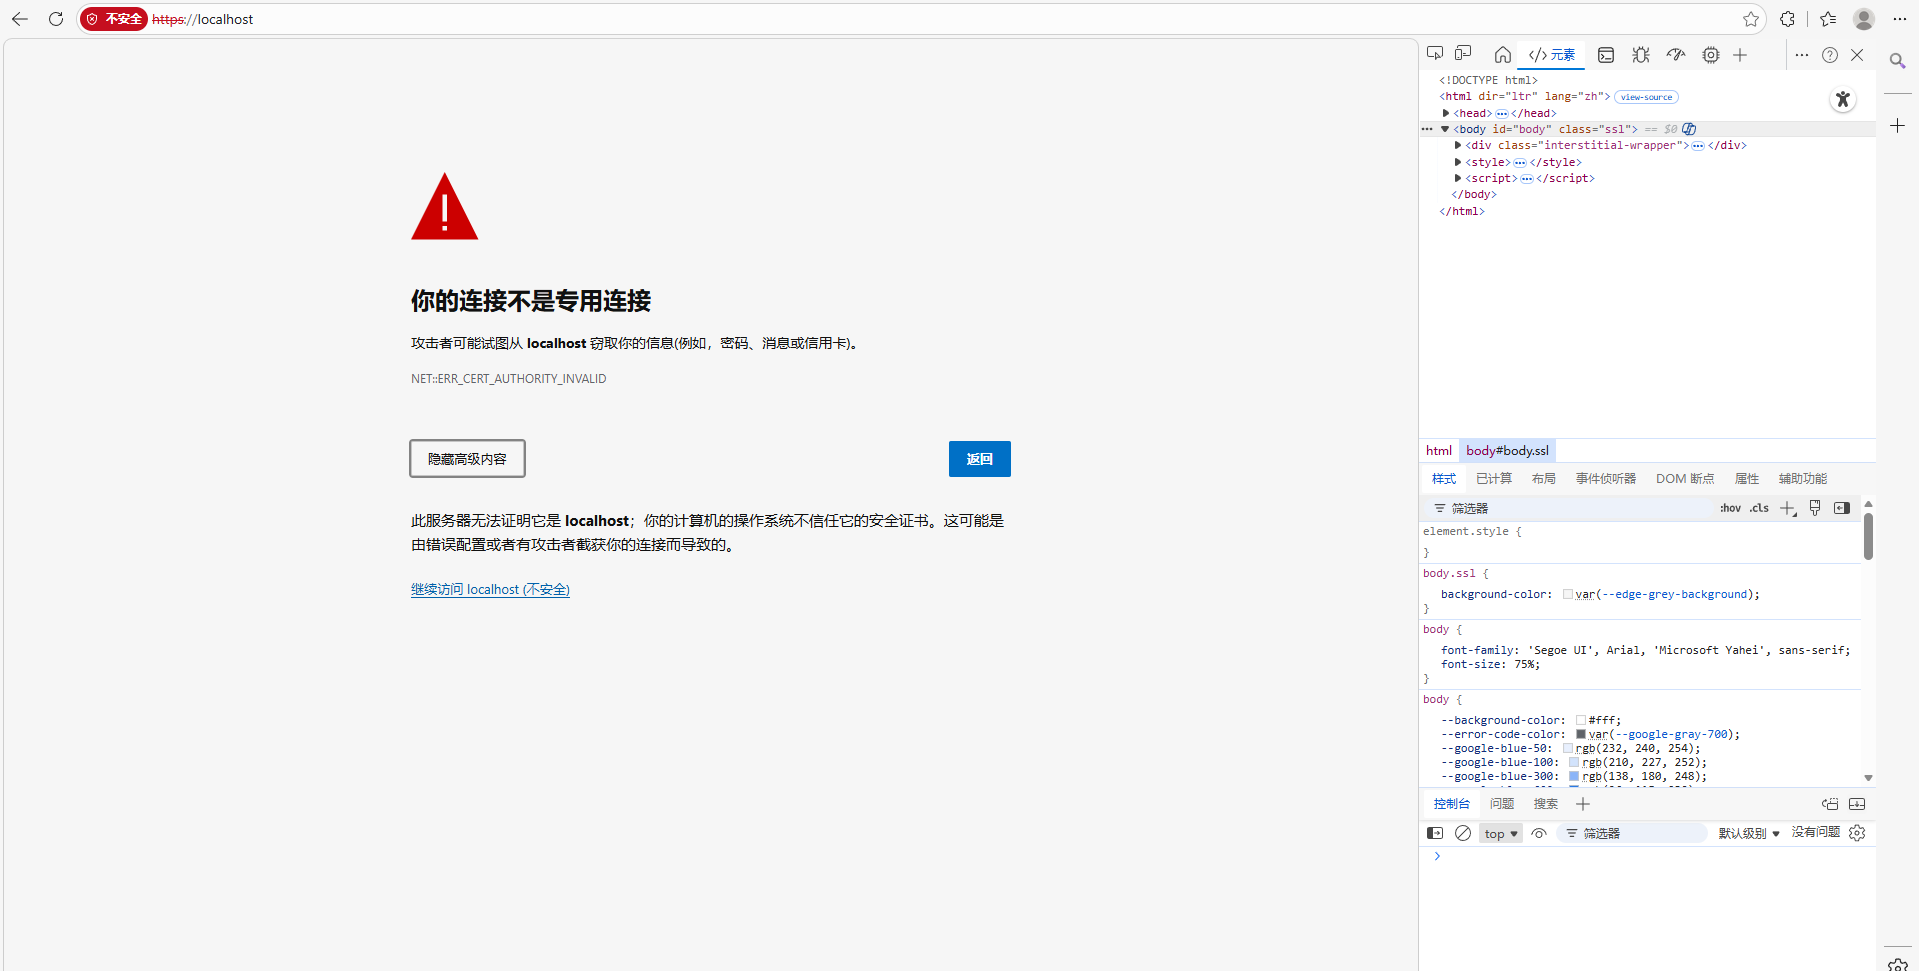
\includegraphics[width=0.6\linewidth]{pngs/warning.png}\\
					\textbf{图6：}浏览器提示安全警告
				\end{center}
			\end{minipage}
			点击“高级” → “继续前往 localhost（不安全）”，即可看到我们设置的测试页面。\\
			\begin{minipage}{\columnwidth}
				\begin{center}
					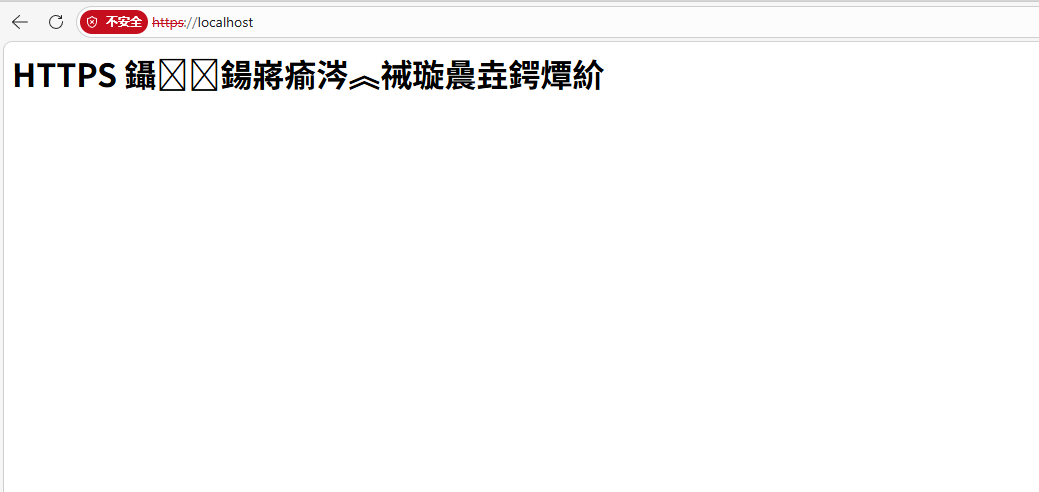
\includegraphics[width=0.6\linewidth]{pngs/error.png}\\
					\textbf{图7：}浏览器展示内容
				\end{center}
			\end{minipage}
			由于本机的Linux虚拟机没有完全安装好中文，所以输出的乱码是正常的情况。之后我们通过浏览器自带的CA查看器就可以查看到我们之前设置的CA证书的详细内容了\\
			\begin{minipage}{\columnwidth}
				\begin{center}
					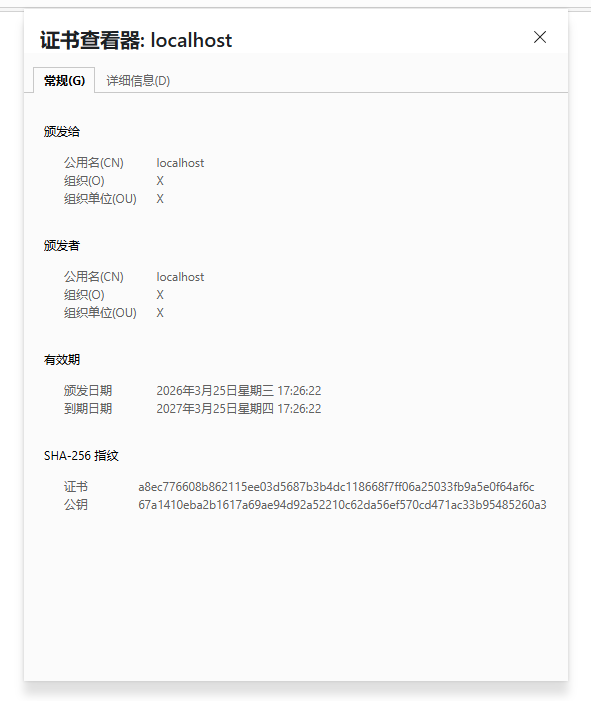
\includegraphics[width=0.4\linewidth]{pngs/webcrt.png}\\
					\textbf{图8：}通过CA查看器得到的效果
				\end{center}
			\end{minipage}
		\end{analogy}
		\section{补充部分}
		最后我实现了自己生成自己的RSA密钥对，并将公钥文件通过国科大邮箱发送给助教老师，然后将助教老师的GPG公钥导入自己的密钥环\\
		\hspace*{2em}\\
		\begin{minipage}{\columnwidth}
			\begin{center}
				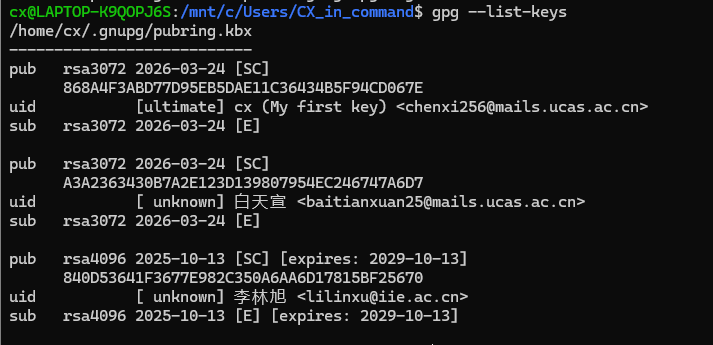
\includegraphics[width=0.6\linewidth]{pngs/gpgimport.png}\\
				\textbf{图9：}导入助教密钥到密钥环\\
				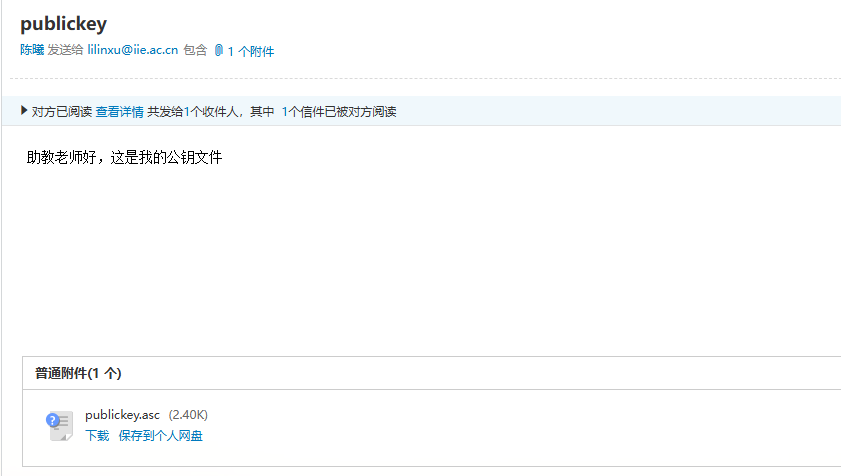
\includegraphics[width=0.6\linewidth]{pngs/keychange.png}\\
				\textbf{图10：}发送自己的公钥文件\\
			\end{center}
		\end{minipage}
		\hspace*{2em}\\
		\hspace*{2em}接下来本文件将会使用助教老师的公钥进行加密本文件。
		\begin{codeblock}{bash}
gpg --recipient lilinxu@iie.ac.cn --sign --encrypt 实验二.pdf
		\end{codeblock}
		\section{结论与总结}
		本实验通过理论分析与工程实践，明确了哈希算法与加密算法在密码学体系中的分工：哈希函数以不可逆性保障数据完整性，加密算法以可逆性保障数据机密性。自签名证书 HTTPS 服务器的搭建验证了数字证书在传输层安全中的关键作用，同时也揭示了自签名证书因缺乏第三方认证而无法通过浏览器安全验证的现实局限。GnuPG 密钥的生成与加密通信实践，完整模拟了非对称加密中密钥分发与加密传输的标准流程。
		
		实验结果表明，现代密码技术已形成“对称加密保障效率、非对称加密解决密钥分发、哈希算法确保完整性”的协同机制。理解各算法的适用边界，是正确构建安全通信系统的前提。本次实验为后续深入学习数字证书体系、公钥基础设施及网络安全协议奠定了实践基础。
	\bibliographystyle{plain}   % 或您需要的样式，如 ieeetr, alpha 等
	\bibliography{reference}
	
\end{document}
